\section{Structure}\label{sec:Structure}
For the simulation environment to be useful, some basic functionality is needed. The simulation should be easy to setup and adjust if needed. 
Furthermore, an easy way to view the result of the simulation is needed such that necessary adjustments can easily be made based on the result.

The first overall thing to consider is the composition of components desired to simulate. 
To make the simulation environment useful it should be able to handle different compositions of pipes and tanks. Meaning that the simulation environment can simulate different setups than the one shown in figure \ref{fig:kloakgrid_simplified}. For this, a simple setup procedure, where different sizes of pipes with different parameters can be chosen, is needed. 
The second thing to consider is that the environment should be brought to a steady state before the simulation starts. The reason for this is that unintended results can arise when working with non-linear systems. Transients caused by the system not to be in a steady state, when starting simulating, can skew the initial data obtained, which is not ideal.   
Also if a linearized approach to the MPC scheme is chosen a linearized model is necessary, which requires a system in steady state to obtain. 
The simulation should be able to run for a predefined amount of iterations. 
Based on this the basic structure of the simulation environment can be split into three parts as shown in figure \ref{fig:struct_overview}.

\begin{figure}[H]
\centering
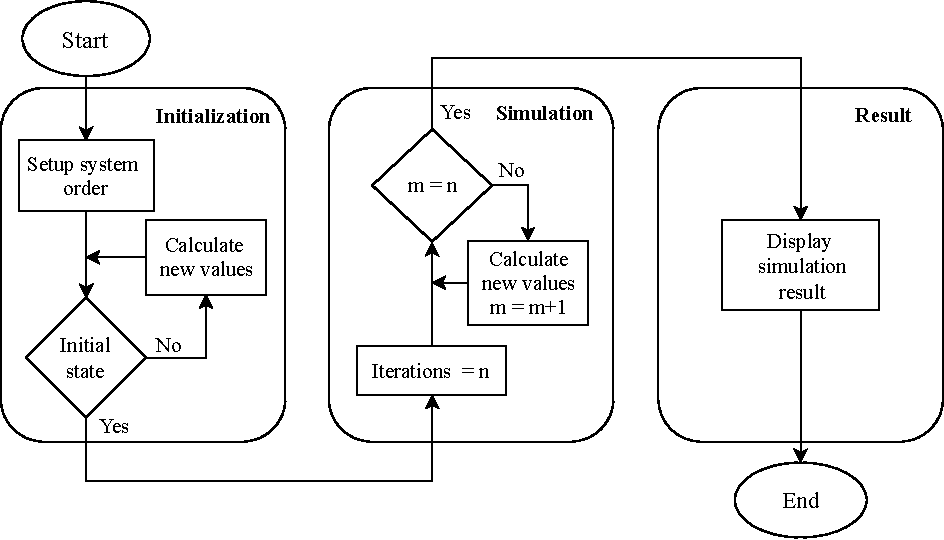
\includegraphics[width=0.9 \textwidth]{report/simulation/pictures/struct_overview_v2.pdf}
\caption{Basic overview of simulation environment}
\label{fig:struct_overview}
\end{figure}


% \begin{enumerate}
% 	\item Initialization
% 	\item Simulation
% 	\item Result
% \end{enumerate}

%To solve the non-linear equations obtained for the free flow channel model in subsection \ref{subse:open_channel} the Preissman scheme is utilized. This scheme is explained in detail in section 
%The following will go into details of the design and the considerations made during the design phase, of the three parts shown in the figure.
The following will go into details, on the thoughts and the considerations made during the design phase, of the three parts shown in the figure.

\subsection*{Initialization} 
The initialization process is, as shown in figure \ref{fig:struct_overview}, comprised of several parts. The first part is to set up the desired system of pipes and tanks such that the system is simulated with the chosen components in the right order.
%As mentioned in section \ref{ch:simulation_solution_and_limitation} a solution to minimize flow and concentrate variations could be insertion of one or more tanks in the sewer network. 
Secondly, the system should be brought in to a steady state from which the simulation can start.
The reason for this is that the Saint-Venant equations utilized to simulate the flow in the sewer pipes is non-linear. Because of this, it can be difficult to find a steady state by hand, which do not produce an unintended result when starting simulating. Though it might be possible to find fitting initial values for small setups it is assumed that a larger setup will increase the chance of unintended results when starting simulating.

For the first part, a simple system setup is decided upon, where the desired components are added to a list. The order of the list then decides how the components is connected when simulating. An example of this setup procedure is shown in figure \ref{fig:sys_setup}. 

\begin{figure}[H]
\centering
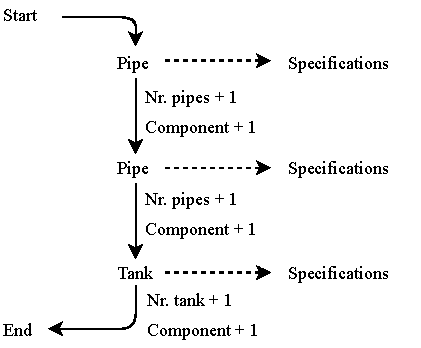
\includegraphics[width=0.5 \textwidth]{report/simulation/pictures/sys_setup.pdf}
\caption{Setup scheme of system order initiation}
\label{fig:sys_setup}
\end{figure}

The specifications for each part in figure \ref{fig:sys_setup} refers to the parameters needed to run the simulation.
The necessary specifications entered for pipe and tank should as a minimum be the required parameters needed to utilize the Preissmann scheme explained in section \ref{se:preissmann_scheme} and to simulate in- and outflow of one or more tanks, respectively. Furthermore, constants which are utilized during simulation should be calculated during initialization such that the computational load is kept as low as possible during simulation. 

A simple solution to bring the desired system setup to an initial steady state is to give a fixed input flow and iterate. 
The iteration continues until a satisfactory error between the fixed input and the flow within the designated setup is deemed sufficiently low. For this to work, it is important to have side input or disturbance input in mind. In figure \ref{fig:simple_sewer} a simple setup is shown of a possible setup to be simulated. 

\begin{figure}[H]
\centering
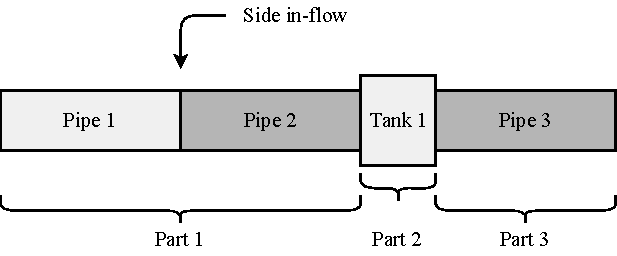
\includegraphics[width=0.55 \textwidth]{report/simulation/pictures/simple_sewer.pdf}
\caption{Simple setup with three pipes, a tank and a single side input}
\label{fig:simple_sewer}
\end{figure}

To make the steady state iteration scheme work on a dynamic level, the components can be separated into parts where adjoint pipes are seen as a single part. The system can then be brought in to steady state one part at a time. As the pipes are the only non-linear part of the system, they are the only parts needed to be iterated upon. Taking the first part in figure \ref{fig:simple_sewer} as an example, there are two pipes and the second one has a side input.
A general expression of the average flow in the parts containing pipes is given by the following equation:

\begin{equation}
 \text{Part-m}_{\text{avg}}	=  \frac{ \sum\limits_{i=1}^n \text{Pipe-input}_i + \text{side inflow}_i }{ n_{\text{pipes}} } 
 \end{equation} \label{avg_init_flow}

Equation \ref{avg_init_flow} can then be used to obtain the desired steady state flow and a current one by utilizing values obtained by solving the Saint-Venant equations. The iteration can then be set to stop when the error between the desired and the measured average is sufficiently low. The next part in figure \ref {fig:simple_sewer} is, in this case, a tank, set to have an in- and outflow equal to the output of the second pipe, which is the combined flow of the first pipe plus the side input. For the third part, the iteration process then starts over with the outflow of the tank as input.
As the concentrate flow is depending on the solution of the Saint-Venant equations it is assumed that when the flow is in a steady state the concentrate will have reached steady state as well.

\subsection*{Simulation}

Having obtained a setup in steady state the next part is to simulate it for the predefined amount of iterations. An important part of the simulation is to store data in a way such that it is easily and intuitively obtainable for purposes such as debugging or customized plots. For this reason, it is decided to store the data, from simulating, into separate blocks. This means that data from individual pipes and tanks should be stored separately in the order given by the initial component setup shown in figure \ref{fig:sys_setup}. In figure \ref{fig:simple_simulation} a simple overview of the simulation procedure is given.   

\begin{figure}[H]
\centering
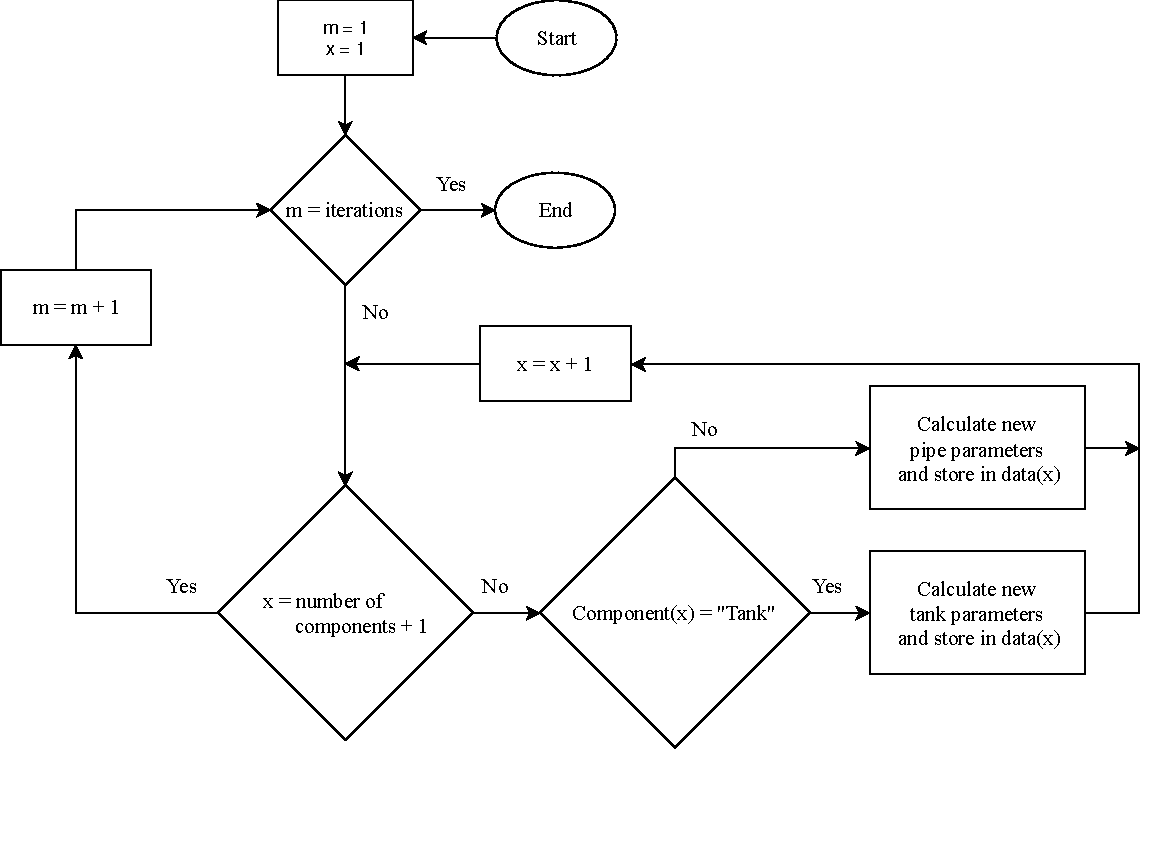
\includegraphics[width=1 \textwidth]{report/simulation/pictures/simple_simulation.pdf}
\caption{Basic overview of the simulation scheme where x indicate an index going from one to the amount of component in the setup and m indicate current iteration.}
\label{fig:simple_simulation}
\end{figure}

The main idea behind the simulation scheme is to calculate one component at a time, and split the calculation of various components into separate functions.
This structure makes it more simple to incorporate new components or insert replacement components if needed further on. A replacement component could e.g. be another scheme to solve the Saint-Venant equations.  

\subsection*{Display result}

Having obtained data from simulating the user-defined system an overview of the results is needed. Considerable time can be spent in designing a function which can display the data in various forms. As the data can consist of a large number of components as well as a considerable time span, it can get quite time consuming to pinpoint parts of interest in time and place. For this reason it is decided that a solution which can give an overview of the obtained data is needed. The chosen solution is a function which can playback the simulated data at a user defined speed and interval. Furthermore, it should be possible to pause and start the playback at a user-defined iteration. Furthermore the chosen areas of interest to be displayed is chosen to be flow, height, concentrate and concentrate flow for pipes. Tanks should when present be shown with a split axis on the right side of the flow, height and concentrate pipe plots.

In figure \ref{fig:display_results} an illustration of the solution is seen.   

\begin{figure}[H]
	\centering
	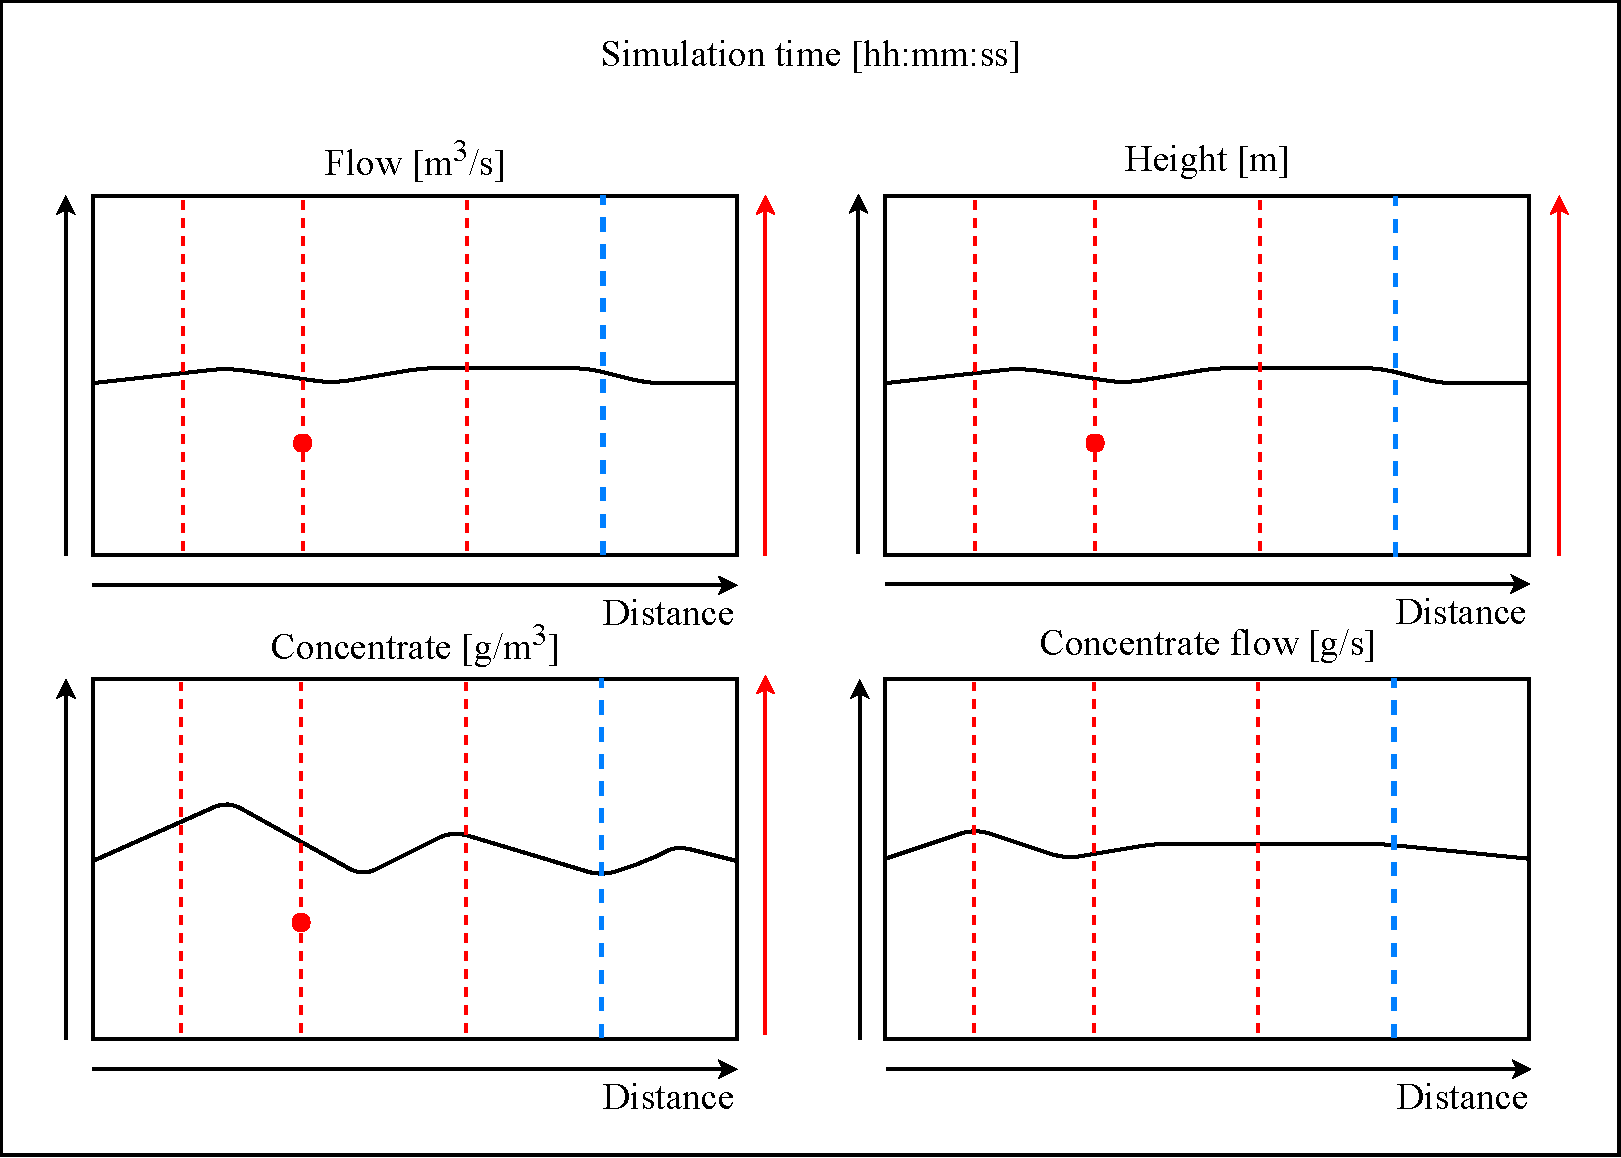
\includegraphics[width=0.95\textwidth]{report/simulation/pictures/display_results}
	\caption{Illustration of the desired visual interface for the playback function where flow, height, concentrate and concentrate flow in the sewer network is seen. The red dashed lines indicates interconnection of pipes, the red dot denotes that a tank is placed at that position and the right y axis indicates height in that tank. The blue dashed line indicate a pipe with side inflow.}
	\label{fig:display_results}
\end{figure}

The visual interface should make it possible with limited effort to examine the simulation data acquired such that verification or adjustments can be made to the constructed setup. 
%This display should give an overview of the simulated data, where the flow, height, concentrate and concentrate flow across a sewer network can be tracked. In the top of the display the simulation time is shown, thereby the user is able to follow the time, if a certain flow profile for the simulated model is used. 
Having outlined the basic details of the construction of the simulation environment the scheme needed to solve the non-linear Saint-Venant equations is explained in detail in the next section. 